\section{Hvordan får man SQL og C\# til at arbejde sammen?}\label{arkitektur}

Vores program taler sammen med en database, da det skal kunne gemme data fra en svend på en byggeplads, som sekretæren hjemme på kontoret skal kunne tilgå.

Derfor er det nødvendigt, at vores program kan tale sammen med databasen beskrevet i afsnit \ref{databasemodellering}.

Programmet taler sammen med databasen ved hjælp af C\# biblioteket System.Data.SqlClient.\cite{sqlclient}
Dette bibliotek giver os adgang til en masse metoder og klasser, deriblandt SqlConnection klassen.
Klassen repræsenterer en forbindelse mellem programmet og en SQL server.
Derfor skal dens constructor tage de nødvendige loginoplysninger: Serveren, hvilken database på serveren, og til sidst brugerens ID og kodeord.

SqlConnection har en metode, der hedder Open(), der åbner forbindelsen til databasen, som er specificeret i SqlConnection constructor.

\subsection{Hvordan henter vi sager fra databasen?}

\begin{figure}[H]
    \makebox[\textwidth][c]{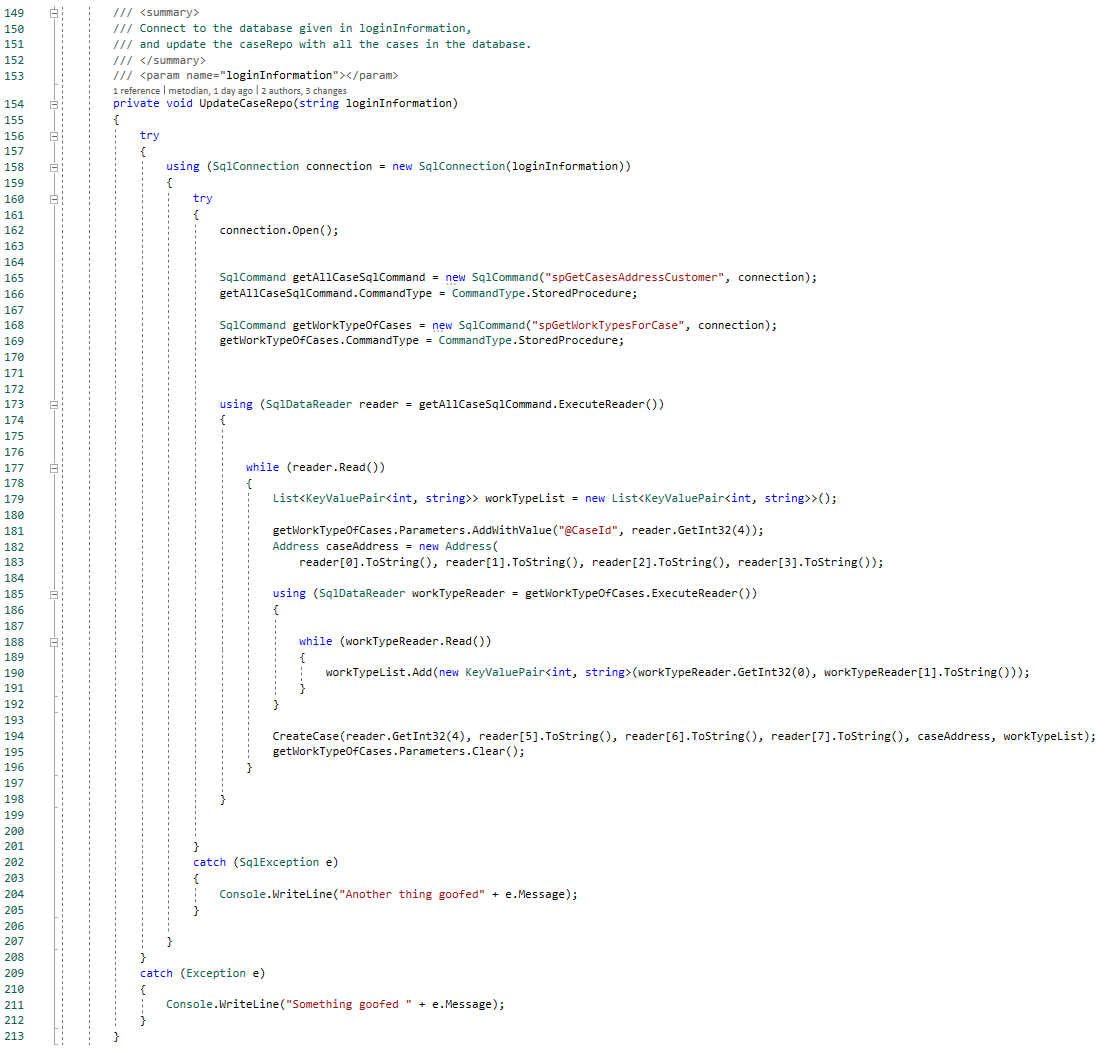
\includegraphics[scale = 0.9]{UpdateCaseRepo.PNG}}
    \caption{Her vises metoden UpdateCaseRepo, som ligger i classen CaseRepo. Denne metoder henter alle cases med til hørende customers og addresses fra databasen.}
    \label{fig:UpdateCaseRepo}
\end{figure}

I figur \ref{fig:UpdateCaseRepo} ser vi opdaterings metoden, som sørger for at hente alle vores cases fra databasen.
UpdateCaseRepo tager som parameter en string.
Denne string indeholder login informationer til den database vi bruger, dette kan ses på linje 154.

Det første vi gør er, at vi bruger en try og catch på SqlConnection, for at se om vi kan lave en forbindele til databasen med den string, metoden bruger.
Hvis den ikke kan lave en SqlConnection fanger catch statementet den exeception, der bliver smidt ud.
I linje 158 bruges der keyworded \textit{using}, som sørger at lukke Sqlconnection igen efter den er færdig med at bruge den, ellers skal metoden Close() bruges for at lukke forbindelen.

Using gør, at det objekt, der står inde paranteserne, kun findes i den følgende kodeblok, ved at den nedlægger objektet ved at kalde objektets Dispose() metode, når kodeblokken er eksekveret.
Derfor skal det objekt, der bruges i using udtrykket implementere IDisposable interfacet.\cite{using}

Efter forbindelsen er blevet åbnet med metoden Open() i linje 162, bliver der lavet to SqlCommands (getAllCasesSqlcommand og getWorkTypeOfCases) fra linje 165 til 169.
Disse to refererer til de to stored procedures med samme navn, som er beskrevet nærmere i afsnit \ref{databasemodellering}.

I linje 173 bliver der brugt en ny using, hvor der bliver oprettet og eksekveret en SqlDataReader på Sqlcommanden getAllCasesSqlcommand.
Efterfølgende bruges der et while loop, som kører hele readeren igennem med metoden Read().
Dette sker på linje 177.
Hver gang reader.Read() bliver kørt bliver der indlæst en række fra databasen ind i reader.
Man tilgår dataen i reader objektet som data i et array.
Inde i dette while loop på linje 179 bliver der oprettet en ny liste workTypeList, som er af typen KeyValuePair.
En list af typen KeyValuePair bruges når man gerne vil associere en nøgle med en værdi.
Dette gør det nemmere at finde ting i listen hvis vi ved hvad nøglen er.

Før den næste SqlCommand getWorkTypeOfCases kan blive kørt, skal der oprettets en ny parameter, som sker på linje 181, denne parameter kommer fra SqlDataReader reader på plads 5.
Hvis du bare tager index nummeret i readeren er den ikke type specifik.
Da vi skal bruge en interger er vi derfor nødtil at bruge metoden GetInt32() for at specificere det.\cite{sqlreader}

Fra linje 181 til 183 bliver der instansieret et nyt address objekt, som får værdier fra SqlDataReader reader fra index 0 til og med index 4.

Efter dette bliver der lavet en ny SqlDataReader, som hedder workTypeReader, men før at vi kan eksekvere to readers i samme connection, skal vi tilføje en ekstra parameter til vores loginInformation string på linje 154, som er \textit{MultipleActiveResultSets=True}.
Inde i denne reader bliver der oprettet og tilføjet nye KeyValuePairs til listen på linje 179, disse KeyValuePairs er worktypes, som den case, der skal oprettes, skal have.

Til sidst før loopet bliver kørt igen, bliver der oprettet et nyt case objeckt med de resterende outputs fra getWorkTypeOfCases og det nye objekt caseAddress på linje 182 og den liste, der er blevet oprettet med SqlDataReader workTypeReader.
For at kunne blive ved med at bruge den stored procedure er man nød til at bruge metoden Clear() til sidst.
Clear() fjerner parameteren der blev tilføjet på linje 181.

Hvis man ikke laver et kald på Clear() metoden vil linje 181 tilføje endnu en parameter, og der vil derfor ske en fejl, når den stored procedure bliver eksekveret, da den ikke kan tage 2 parametre.
